% !TeX root = ../solution.tex

\hypertarget{he22.15}{%
\chapter{[HE22.15] LEDs}\label{he22.15}}

\begin{marginfigure}
	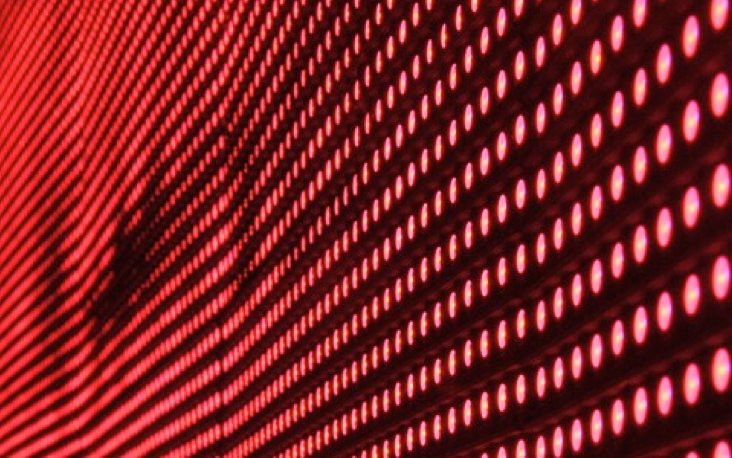
\includegraphics[width=50mm]{level4/challenge15.jpg}
\end{marginfigure}
\subsection{Intro}
I got this hex dump, but I don't know what it is.

\noindent Any idea?

\noindent File: \verb+leds.hex+

\section{Solution}\label{hv22.15solution}
The file is a variant of the Intel hex file format (see \url{https://en.wikipedia.org/wiki/Intel_HEX}.  On the second line a record type is given as 0x0A, which seems to be used in the BBCMicro:bit computer.  At \url{https://makecode.microbit.org/#editor} we can find an emulator that can show the code as JavaScript code

\begin{minted}{javascript}
input.onButtonPressed(Button.A, function () {
    j += 0 - 1
})
input.onButtonPressed(Button.AB, function () {
    basic.showString("" + (scribble(c)))
})
input.onButtonPressed(Button.B, function () {
    j += 5
})
function scribble (s: string) {
    for (let i = 0; i <= s.length - 1; i++) {
        r = "" + r + String.fromCharCode(s.charCodeAt(i) + j)
    }
    return r
}
let r = ""
let j = 0
let c = ""
c = "ZW$\"$$m`%&fQ^#ff^%QV%h#U%o"
\end{minted}

So the characters in string c are shifted by an amount to print the flag.  Looking at c, we can make an educated guess that ``\$''\$\$´´ will be turned into ``2022´´ and thus a small python script prints the flag \verb+he2022{n34t_l1ttl3_d3v1c3}+.
\begin{minted}{python}
s = ord('2') - ord('$')
flag = ''
for c in 'ZW$"$$m`%&fQ^#ff^%QV%h#U%o':
     flag += chr(ord(c)+s)

flag
\end{minted}






